\section{Bluetooth Low Energy}

\begin{frame}
	\frametitle{Bluetooth Low Energy}
	\begin{minipage}[t]{0.66\linewidth}
		\vspace{0.5cm}
		\center{\Large{Services}}
		\vspace{0.5cm}
		\begin{itemize}
			\item "Healthcare"
			\item "Fitness"
			\item "Human Interface Device"
			\item "Alert"
			\item "Proximity"
			\item Capteurs génériques
			\item Découverte de services
			\item Et bien plus...
		\end{itemize}
	\end{minipage}
	\begin{minipage}[t]{0.30\linewidth}
		\vspace{0.5cm}
		\begin{block}{Radio}
			\begin{itemize}
				\item 2.4 GHZ
				\item 40 canaux
			\end{itemize}
		\end{block}
	\end{minipage}
\end{frame}

\begin{frame}
	\frametitle{Stack BLE}
	\begin{minipage}{0.45\linewidth}
		\begin{figure}
			\includegraphics[height=6cm]{img/HCI_GATT.png}
		\end{figure}
	\end{minipage}
	\begin{minipage}{0.50\linewidth}
		\begin{block}{Stack Bluetooth Low Energy}
			\begin{itemize}
				\item Link Layer
				\item L2CAP
				\item Protocole ATT
				\item Profile GATT
				\item Services : Application
			\end{itemize}
		\end{block}
	\end{minipage}
\end{frame}

\begin{frame}
	\frametitle{Link Layer}
	\begin{minipage}{0.60\linewidth}
		\begin{figure}
			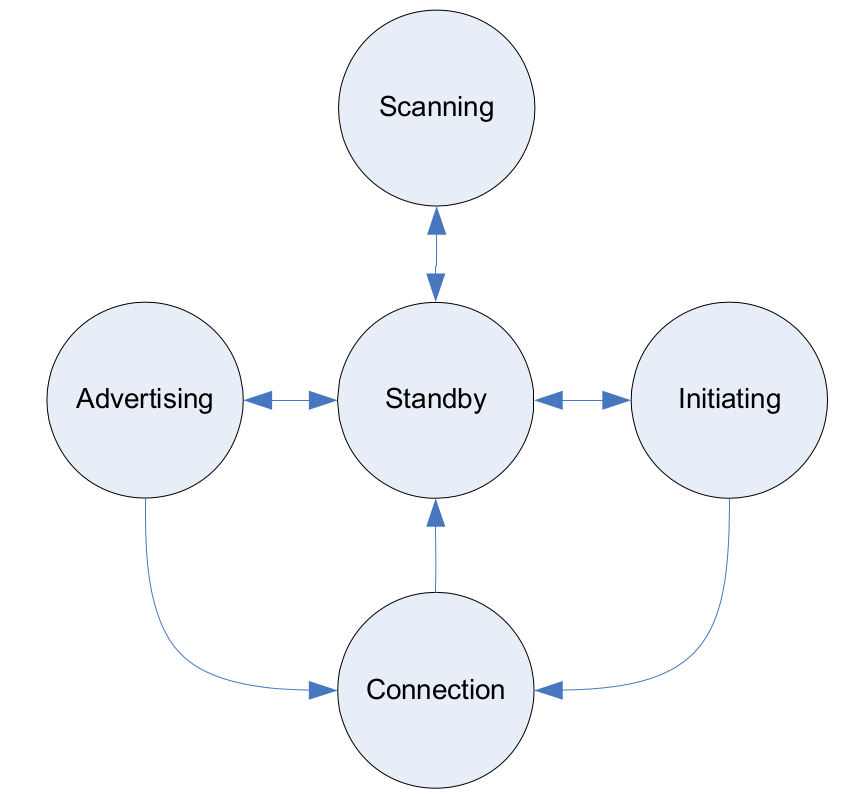
\includegraphics[height=6cm]{img/BLE_LL.png}
		\end{figure}
	\end{minipage}
	\begin{minipage}{0.35\linewidth}
		\begin{itemize}
			\item<1-> Idle \\ {\tiny{On ne fait rien}}
			\item<2-> Advertising \\ {\tiny{Broadcast, connectable ou non}}
			\item<3-> Scanning \\ {\tiny{Ecoute d'advertisements}}
			\item<4-> Initiating \\ {\tiny{Ecoute d'advertisements}} \\
								{\tiny{Réponse par connexion}}
			\item<5-> Connection \\ {\tiny{Connecté}} \\
				{\tiny{Master (depuis Initiating) ou}} \\
				{\tiny{Slave (Depuis Advertising)}}
		\end{itemize}
	\end{minipage}
\end{frame}


